\chapter{\label{ch3-architecture}CTA Architecture} 

\minitoc

\notes[inline,caption={}]{
	\section{Plan}
	\subsection{Topics}
	\begin{itemize}
		\item Requirements
		\item Data Levels
	\end{itemize}
	\subsection{Questions}
	\begin{itemize}
		\item ?
	\end{itemize}
}

\section{Introduction}

Due to the large scope of \gls{cta}, in both its construction and operation, a formal approach towards a system architecture was adopted . One important aspect of this architecture is the distinction between the \gls{cta} Observatory and the \gls{cta} Consortium. 

\section{CTA Consortium and Observatory

\section{Requirements}



Telescopes, cameras, and other products designed for \gls{cta} must adhere to the 

test

\begin{requirement}{B-TEL-1010 Charge Resolution}
	The required fractional Charge Resolution for Cherenkov signals in each Camera pixel for a specified background level of 0.125 photoelectrons/ns is given in the Figure below and Table attached. Charge measurements must be possible for 0-1000 photoelectron signals. The average charge resolution should be calculated for the reference Gamma-Ray Spectrum.
    
	\centering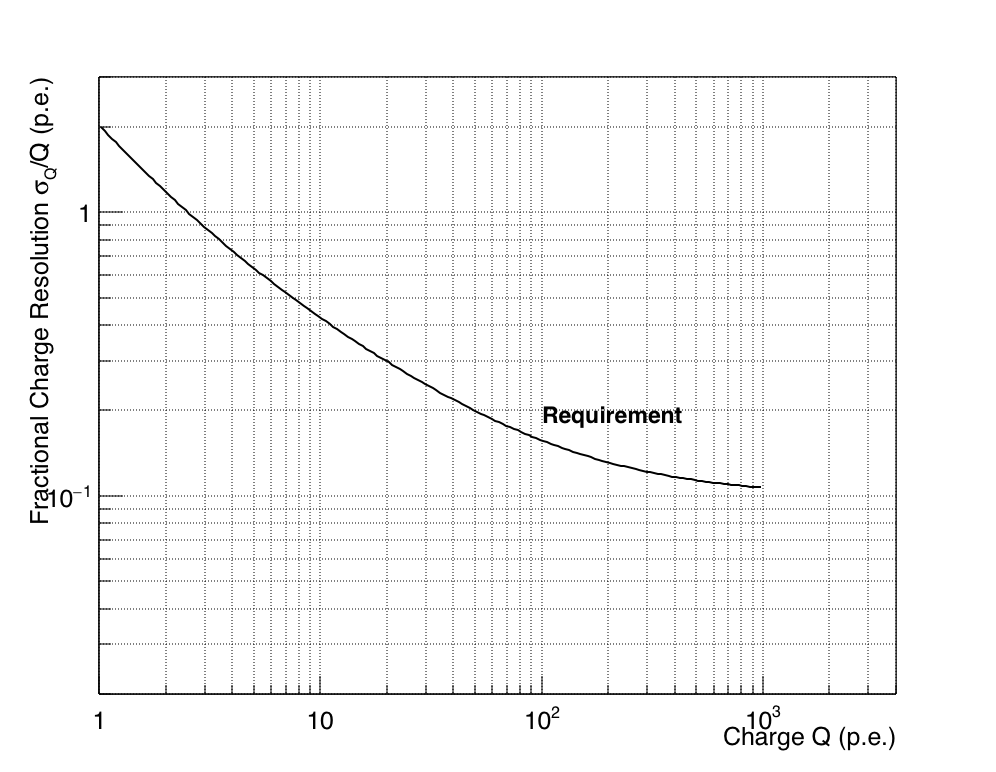
\includegraphics[width=0.8\linewidth]{figures/images/charge_res_req}
	\captionof{figure}{Fractional rms charge resolution $\sigma_Q/Q$ per pixel for different Cherenkov light signal amplitudes, expressed in units of photoelectrons (p.e.). All sources of fluctuations, including Poisson fluctuations in photoelectron number, must be included, The true pixel charge $Q$ is that measured in an ideal detector with the same photon-detection efficiency. }\label{fig:charge_res_req}
    
\begin{itemize}
\item [Notes:] It is expected that this requirement is verified with reference to:

- Monte Carlo simulation of Cherenkov light from gamma-ray initiated showers (using a verified telescope model),

- Level-C Specification on Laboratory Measured Charge Resolution,

- Monte Carlo simulation of the laboratory test set-up (as a means of telescope model verification).

Note that between 1000pe and 2000pe, some sensitivity to increasing input signal must exist. \newline
This requirement applies to post-calibration (DL1) data. \newline
Note that this requirement will likely need to be expanded to cover performance at higher NSB levels.
\end{itemize}
\end{requirement}

\section{Data Levels}